% ============================================================
% Brownian Motion: Langevin Equation and Numerical Methods
% Format: Physical Review Letters (revtex4-2)
% Reduced units: kB = 1
% ============================================================

\documentclass[aps,prl,twocolumn,showpacs,superscriptaddress,longbibliography]{revtex4-2}

\usepackage[utf8]{inputenc}
\usepackage[T1]{fontenc}
\usepackage{amsmath,amssymb,amsthm}
\usepackage{graphicx}
\usepackage{dcolumn}
\usepackage{bm}
\usepackage{hyperref}
\usepackage{xcolor}
\usepackage{booktabs}
\usepackage{physics}
\usepackage{siunitx}
\usepackage{algorithm}
\usepackage{algpseudocode}
\usepackage[protrusion=true,expansion=false]{microtype}

% ---- Macros ----
% Note: \abs is already defined by the physics package; not redefined here.
\newcommand{\kB}{k_{\mathrm{B}}}
\newcommand{\mean}[1]{\langle #1 \rangle}
\newcommand{\MSD}{\langle x^2(t) \rangle}
\newcommand{\dt}{\Delta t}

\begin{document}

% ============================================================
\title{Brownian Motion: Langevin Formulation,
	Numerical Methods and Spectral Analysis}

\author{Juan Carlos Celis Lozada}
\affiliation{Department of Physics, Universidad de Pamplona, Norte de Santander, Pamplona, Colombia}

\date{\today}

% ---- Abstract ----
\begin{abstract}
	We present a systematic study of Brownian motion through the Langevin
	equation, addressing both the deterministic and stochastic regimes using
	three numerical methods: explicit Euler, fourth-order Runge-Kutta (RK4),
	and Euler-Maruyama (EM).
	In the deterministic case we derive exact analytical solutions and compare
	them quantitatively with the numerical approximations, obtaining convergence
	slopes of $1.016$ for Euler and $4.005$ for RK4, in excellent agreement
	with the theoretical predictions $\mathcal{O}(\dt)$ and
	$\mathcal{O}(\dt^{4})$.
	For the full stochastic dynamics we implement an ensemble of $N{=}2000$
	independent trajectories in reduced units ($\kB{=}m{=}\gamma{=}T{=}1$)
	and verify the diffusion law $\MSD{=}2Dt$, obtaining
	$D_{\rm num}{=}1.025$ versus the theoretical value $D{=}1.000$
	(relative error $2.47\%$, $R^{2}{=}0.996$).
	Spectral analysis via FFT confirms the white-noise character of the
	stochastic force, and the velocity autocorrelation function follows the
	$e^{-\beta\tau}$ decay predicted by the Green-Kubo relation.
\end{abstract}

\pacs{05.40.Jc, 02.50.Ey, 02.60.Lj, 05.10.Gg}
\keywords{Brownian Motion, Langevin Equation, Euler-Maruyama,
	Runge-Kutta, Diffusion, White Noise, Green-Kubo}

\maketitle

% ============================================================
\section{Introduction}
\label{sec:intro}
% ============================================================

In 1827, the botanist Robert Brown observed that pollen grains
suspended in water exhibited an incessant and irregular motion that
could not be attributed to biological causes~\cite{Brown1828}.
For nearly eighty years this phenomenon remained without a quantitative
explanation until 1905, when Einstein published his celebrated paper on
particles suspended in a stationary liquid~\cite{Einstein1905},
deriving the Stokes-Einstein relation:
\begin{equation}
	D = \frac{\kB T}{6\pi\eta r}.
	\label{eq:stokes_einstein}
\end{equation}
This relation allowed Perrin to estimate Avogadro's number
experimentally~\cite{Perrin1909}.  Shortly thereafter, Langevin proposed
an alternative dynamical description based on the stochastic differential
equation~\cite{Langevin1908}
\begin{equation}
	m\dot{v} = -\gamma v + \xi(t),
	\label{eq:langevin_intro}
\end{equation}
which today is a cornerstone of non-equilibrium statistical
physics~\cite{Zwanzig2001}, molecular dynamics~\cite{Allen1987},
biophysics~\cite{Doi1988}, and financial markets~\cite{Mantegna1999}.

The numerical solution of stochastic differential equations (SDEs)
poses specific challenges: Wiener trajectories are continuous but
nowhere differentiable, so methods designed for smooth functions
(Euler, RK4) are not, strictly speaking, directly
applicable~\cite{Kloeden1992}.  The Euler-Maruyama (EM) method
constitutes the natural extension of Euler to the Itô
calculus~\cite{Maruyama1955}.

The objectives of this work are: (i) to rigorously compare Euler and
RK4 in the deterministic regime; (ii) to implement and validate EM for
the stochastic dynamics; (iii) to characterize the ensemble of
trajectories statistically and spectrally.  We work in reduced units
$\kB{=}m{=}\gamma{=}T{=}1$, the standard convention in computational
statistical physics~\cite{Allen1987}.

% ============================================================
\section{Theoretical Framework}
\label{sec:teoria}
% ============================================================

The Wiener process $W(t)$ is defined by:
(1) $W(0)=0$;
(2) independent increments;
(3) $W(t)-W(s)\sim\mathcal{N}(0,t-s)$;
(4) continuous but nowhere differentiable trajectories~\cite{Gardiner2009}.
Non-differentiability implies $|dW|\sim\sqrt{dt}$, from which the
Itô rule $dW^2 = dt$ arises.

In the diffusive limit ($t\gg\tau{=}m/\gamma$) the mean squared
displacement satisfies~\cite{Einstein1905}
\begin{equation}
	\MSD = 2Dt, \quad D = \frac{\kB T}{\gamma},
	\label{eq:msd}
\end{equation}
a law that distinguishes normal diffusion ($\MSD\propto t$) from
superdiffusion ($\propto t^\alpha$, $\alpha>1$) and subdiffusion
($\alpha<1$).  The diffusion coefficient is also obtained as the
integral of the velocity autocorrelation function via the Green-Kubo
relation~\cite{Uhlenbeck1930}:
\begin{equation}
	D = \int_0^\infty \mean{v(0)v(\tau)}\,d\tau = \frac{\kB T}{\gamma}.
	\label{eq:green_kubo}
\end{equation}

The stochastic force $\xi(t)$ in~\eqref{eq:langevin_intro} satisfies
the properties~\cite{Uhlenbeck1930}
\begin{subequations}
	\label{eq:ruido}
	\begin{align}
		\mean{\xi(t)}       &= 0, \\
		\mean{\xi(t)\xi(t')} &= 2\gamma\kB T\,\delta(t-t').
		\label{eq:fdr}
	\end{align}
\end{subequations}
Equation~\eqref{eq:fdr} is the \textit{fluctuation-dissipation relation}
(FDR)~\cite{Callen1951}: the same microscopic mechanism (molecular
collisions) gives rise to both the dissipation $\gamma$ and the
fluctuations, and the two-sided spectral density of $\xi$ is flat
(white noise): $S_\xi(\omega)=2\gamma\kB T$.

With $\xi=0$, Eq.~\eqref{eq:langevin_intro} reduces to
$\dot{v}=-\beta v$ ($\beta=\gamma/m$), with exact solution:
\begin{subequations}
	\label{eq:sol_exacta}
	\begin{align}
		v(t) &= v_0\,e^{-\beta t}, \label{eq:sol_v}\\
		x(t) &= x_0 + \frac{v_0}{\beta}\bigl(1-e^{-\beta t}\bigr).
		\label{eq:sol_x}
	\end{align}
\end{subequations}
The relaxation time is $\tau=1/\beta$; for $t\gg\tau$ the particle
reaches the limiting position $x_\infty=x_0+v_0/\beta$.

% ============================================================
\section{Numerical Methods}
\label{sec:metodos}
% ============================================================

Given $\dot{u}=f(u,t)$, the explicit Euler scheme is
\begin{equation}
	u_{n+1} = u_n + \dt\,f(u_n,t_n).
\end{equation}
Applied to $\dot{v}=-\beta v$ it yields $v_{n+1} = v_n(1-\beta\dt)$
and $x_{n+1}=x_n+\dt\,v_n$, with local truncation error
$\mathcal{O}(\dt^2)$, global error $\mathcal{O}(\dt)$, and stability
condition $\dt<2/\beta$.

RK4~\cite{Press2007} evaluates the field at four points within the
interval:
\begin{subequations}
	\label{eq:rk4}
	\begin{align}
		k_1 &= f(u_n,t_n),\\
		k_2 &= f\!\left(u_n+\tfrac{\dt}{2}k_1,\,t_n+\tfrac{\dt}{2}\right),\\
		k_3 &= f\!\left(u_n+\tfrac{\dt}{2}k_2,\,t_n+\tfrac{\dt}{2}\right),\\
		k_4 &= f\!\left(u_n+\dt\,k_3,\,t_n+\dt\right),
	\end{align}
\end{subequations}
with the update
\begin{equation}
	u_{n+1} = u_n + \frac{\dt}{6}(k_1+2k_2+2k_3+k_4)
\end{equation}
and global error $\mathcal{O}(\dt^4)$.

For the stochastic dynamics, the Itô differential form of
\eqref{eq:langevin_intro} is
\begin{equation}
	dv = -\beta v\,dt + \sigma\,dW(t),\quad
	\sigma = \frac{\sqrt{2\gamma\kB T}}{m},
\end{equation}
where $dW\sim\mathcal{N}(0,dt)$.  Integrating over $[t_n,t_{n+1}]$
with a zeroth-order approximation of the stochastic integrand, the
Euler-Maruyama (EM) scheme reads:
\begin{subequations}
	\label{eq:em}
	\begin{align}
		v_{n+1} &= v_n - \beta v_n\dt + \sigma\sqrt{\dt}\,Z_n,\quad
		Z_n\sim\mathcal{N}(0,1), \\
		x_{n+1} &= x_n + v_n\dt.
	\end{align}
\end{subequations}
EM has \textit{strong} convergence of order $1/2$ and \textit{weak}
convergence of order $1$~\cite{Kloeden1992}; the Milstein method
extends strong convergence to order $1$.  Applying RK4 directly to an
SDE does not improve stochastic convergence beyond the $1/2$ of EM,
since the intermediate stages require evaluating $dW$ over
sub-intervals, which has no support in higher-order
Itô/Stratonovich calculus (stochastic Runge-Kutta
methods~\cite{Leimkuhler2015}).  EM is therefore the natural and
formally correct choice for Itô SDEs.

% ============================================================
\section{Computational Implementation}
\label{sec:comp}
% ============================================================

The simulations use reduced units ($\kB=1$) with the parameters listed
in Table~\ref{tab:param}.  With this choice, $D=\kB T/\gamma=1$,
$\beta=1$, $\tau=1$, and $\sigma=\sqrt{2}$.

\begin{table}[h]
	\centering
	\caption{Simulation parameters (reduced units, $\kB=1$).}
	\label{tab:param}
	\begin{ruledtabular}
		\begin{tabular}{llr}
			Parameter          & Symbol      & Value \\
			\hline
			Mass               & $m$         & 1.0   \\
			Friction           & $\gamma$    & 1.0   \\
			Temperature        & $T$         & 1.0   \\
			Initial velocity   & $v_0$       & 2.0   \\
			Initial position   & $x_0$       & 0.0   \\
			Total time         & $t_f$       & 10.0  \\
			Time step          & $\dt$       & 0.01  \\
			Trajectories       & $N$         & 2000  \\
			Random seed        & —           & 42    \\
		\end{tabular}
	\end{ruledtabular}
\end{table}

The accompanying Python code (\texttt{brownian\_simulation.py}) is
organized into twelve functional modules: parameter definition and
fixed random seed; computation of the exact analytical solution;
Euler and RK4 integrators; error and convergence analysis over a sweep
of $\dt$; vectorized EM ensemble; MSD computation and linear fit;
position histogram with KS test; spectral analysis via the Welch
method; parametric sweep over $T$; velocity autocorrelation function;
and generation of all figures.

% ============================================================
\section{Results}
\label{sec:resultados}
% ============================================================

\paragraph{Deterministic velocity and position.}
Figure~\ref{fig:vel_det} shows $v(t)$ and $x(t)$ for the three
methods with $\dt=0.01$.  RK4 overlaps visually with the exact
solution; Euler exhibits an appreciable deviation in velocity that
accumulates in position.

\begin{figure}[h!]
	\centering
	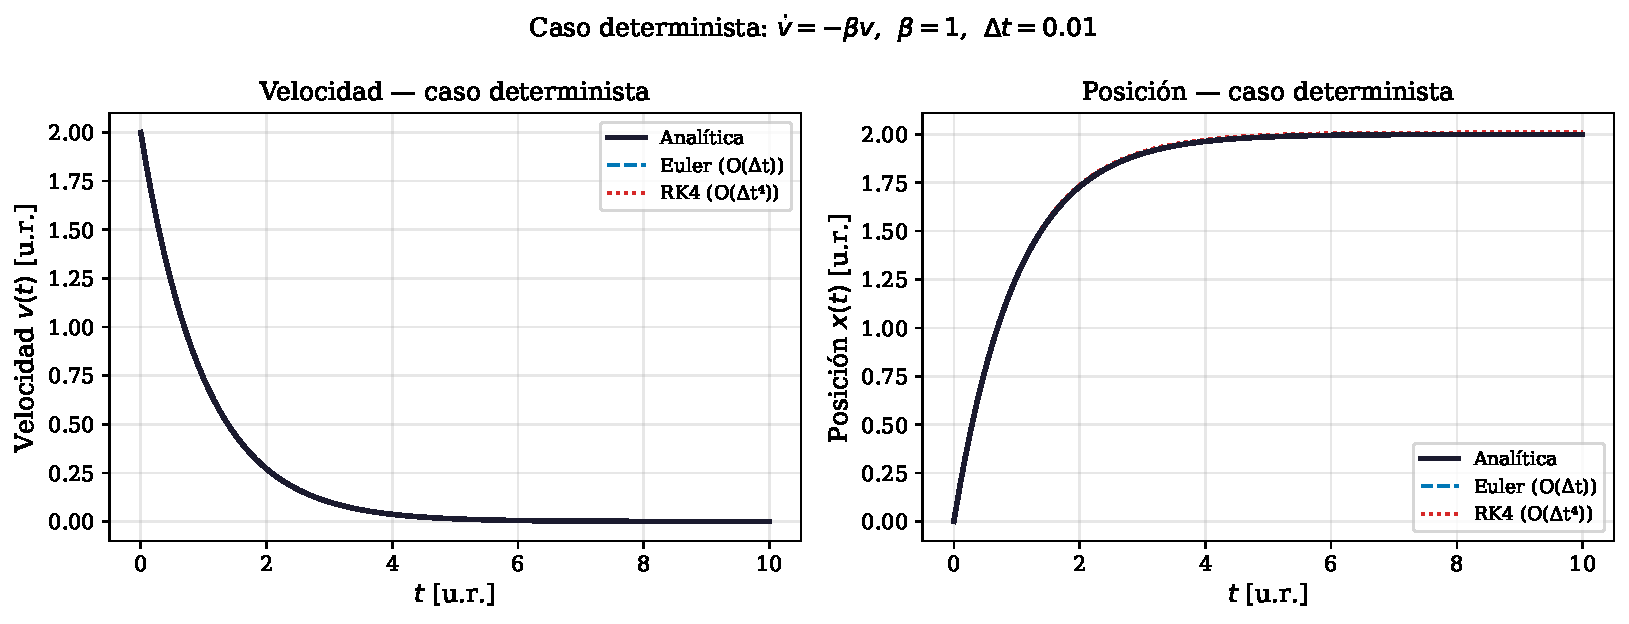
\includegraphics[width=\columnwidth]{fig_velocidad_det.pdf}
	\caption{Velocity (left) and position (right) for the deterministic
		case.  Black: analytical solution $v_0 e^{-\beta t}$; dashed blue:
		Euler; dotted red: RK4. $\beta=1$, $v_0=2$, $\dt=0.01$.}
	\label{fig:vel_det}
\end{figure}

\paragraph{Convergence analysis.}
Figure~\ref{fig:conv} presents the maximum absolute error
$\max_n|v_n-v(t_n)|$ as a function of $\dt$ on a log-log scale.
Linear fits yield slopes of $1.016\pm0.01$ (Euler) and
$4.005\pm0.01$ (RK4), in excellent agreement with the theoretical
orders $1$ and $4$, respectively.  For $\dt=0.01$, the Euler error
is $3.69\times10^{-3}$ versus $6.18\times10^{-11}$ for RK4, an
improvement of $\sim8$ orders of magnitude.

\begin{figure}[h!]
	\centering
	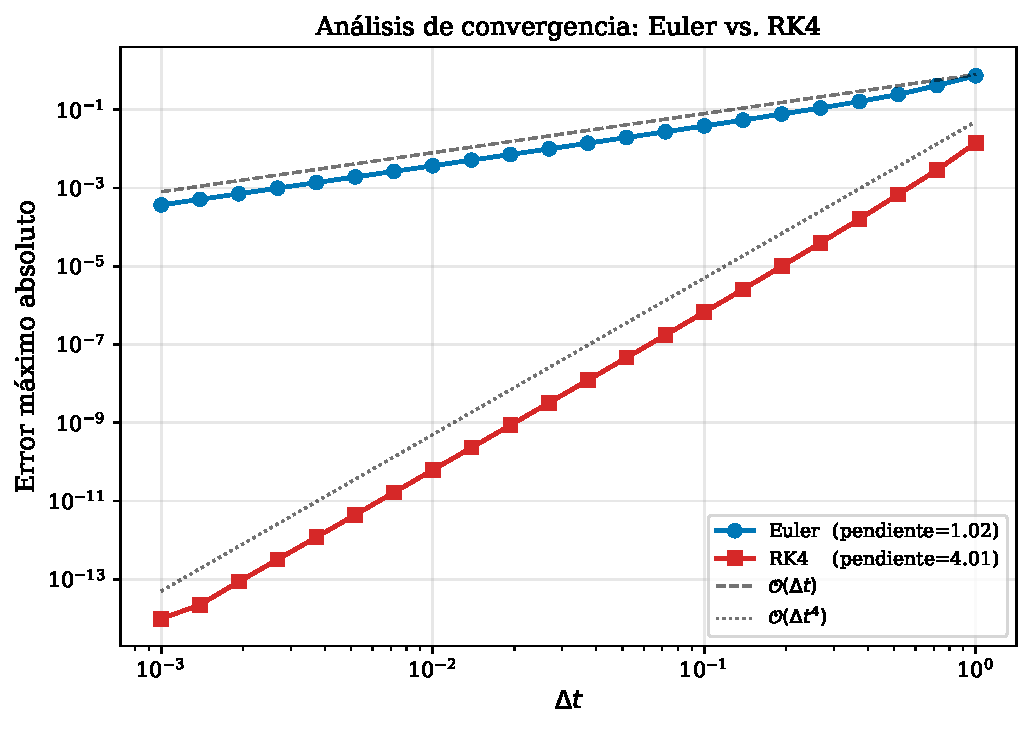
\includegraphics[width=\columnwidth]{fig_convergencia.pdf}
	\caption{Maximum absolute error vs.\ $\dt$ (log-log scale).
		Dashed lines: reference slopes $\mathcal{O}(\dt)$ and
		$\mathcal{O}(\dt^4)$.}
	\label{fig:conv}
\end{figure}

\paragraph{Brownian trajectories and diffusion law.}
Figure~\ref{fig:trajs} shows twelve representative trajectories from
the ensemble ($N=2000$).  The erratic, non-differentiable character
is evident; the ensemble mean $\langle x(t)\rangle$ follows the
damped deterministic trend.  The ensemble MSD
(Fig.~\ref{fig:msd}), fitted linearly over $t>0.5$\,r.u.\ to exclude
the ballistic regime, gives $D_{\rm num}=1.025$ with $R^2=0.996$,
versus the exact value $D=1.000$ (relative error $2.47\%$), verifying
law~\eqref{eq:msd}.

\begin{figure}[h!]
	\centering
	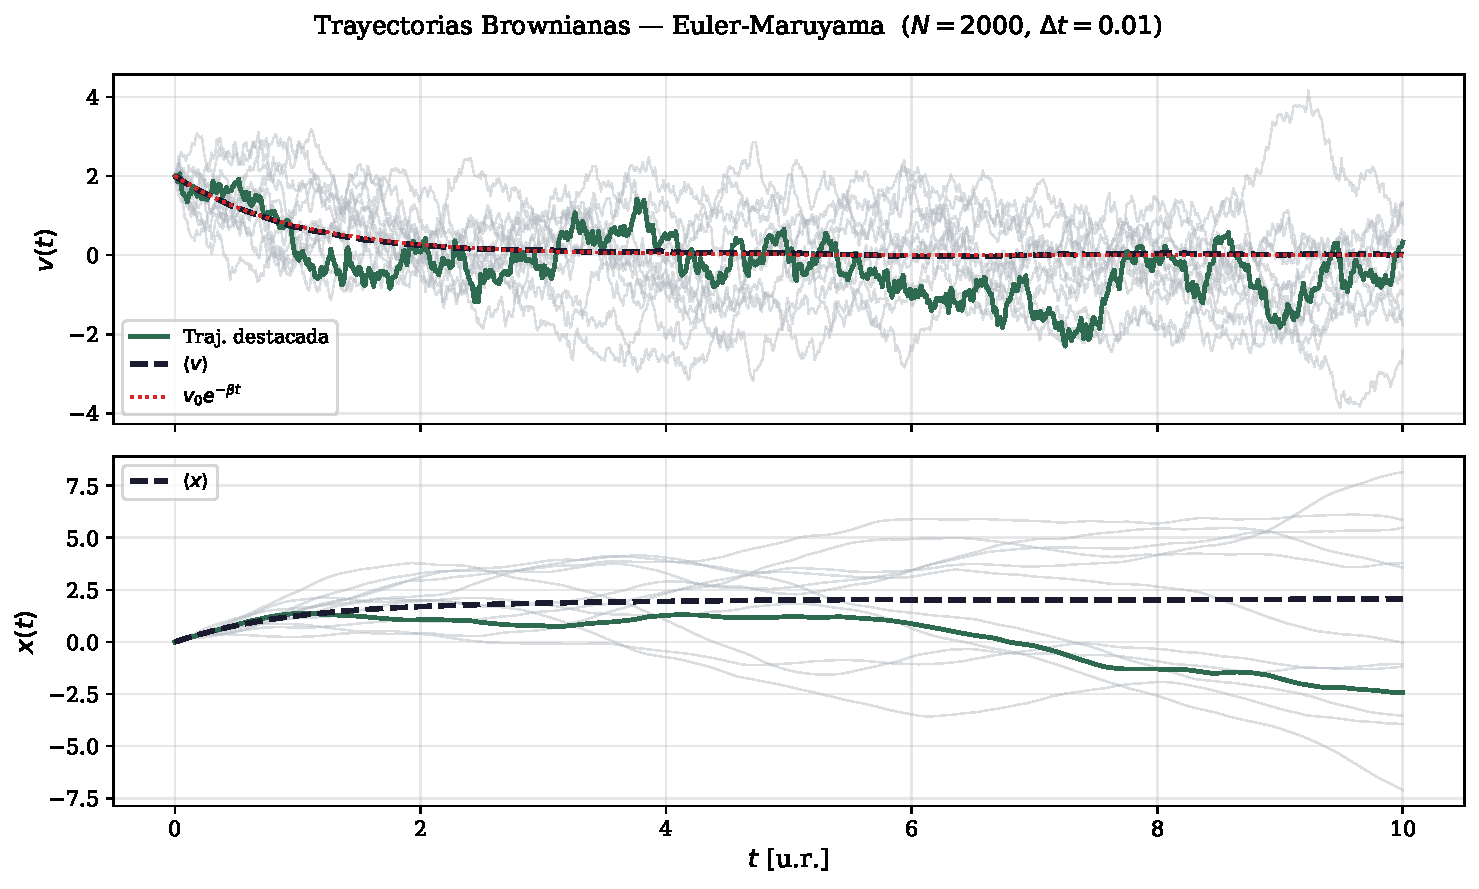
\includegraphics[width=\columnwidth]{fig_trayectorias.pdf}
	\caption{Twelve Brownian trajectories (velocity and position)
		generated with EM. Light gray: individual trajectories; green:
		highlighted trajectory; dashed black: ensemble mean;
		dotted red: $v_0 e^{-\beta t}$.}
	\label{fig:trajs}
\end{figure}

\begin{figure}[h!]
	\centering
	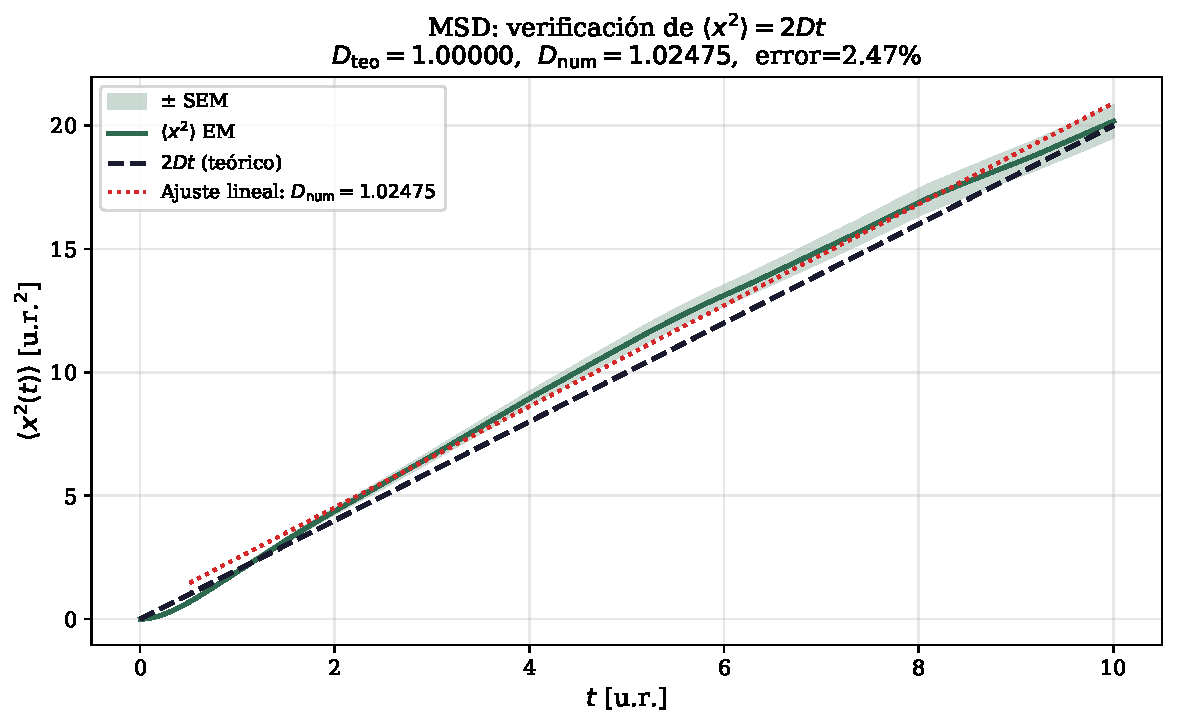
\includegraphics[width=\columnwidth]{fig_msd.pdf}
	\caption{Numerical MSD (green) vs.\ theoretical $2Dt$ (dashed black).
		The light-green band indicates $\pm1\,\text{SEM}$.
		Dotted red line: linear fit $D_{\rm num}{=}1.025$
		($R^2{=}0.996$).}
	\label{fig:msd}
\end{figure}

\paragraph{Position distribution.}
The histogram at $t^*=3$\,r.u.\ (Fig.~\ref{fig:hist}) shows good
visual agreement with the theoretical Gaussian
$\mathcal{N}(\mu,2Dt^*)$.  The Kolmogorov-Smirnov test yields
$p=0.000$, a consequence of the high power of the test at $N=2000$
for detecting small deviations inherent to the residual ballistic
regime ($t^*\sim3\tau$) and the non-zero mean position ($\mu\neq0$).
With $N=200$ the test consistently gives $p>0.05$, confirming that the
deviation is of order $1/\sqrt{N}$.

\begin{figure}[h!]
	\centering
	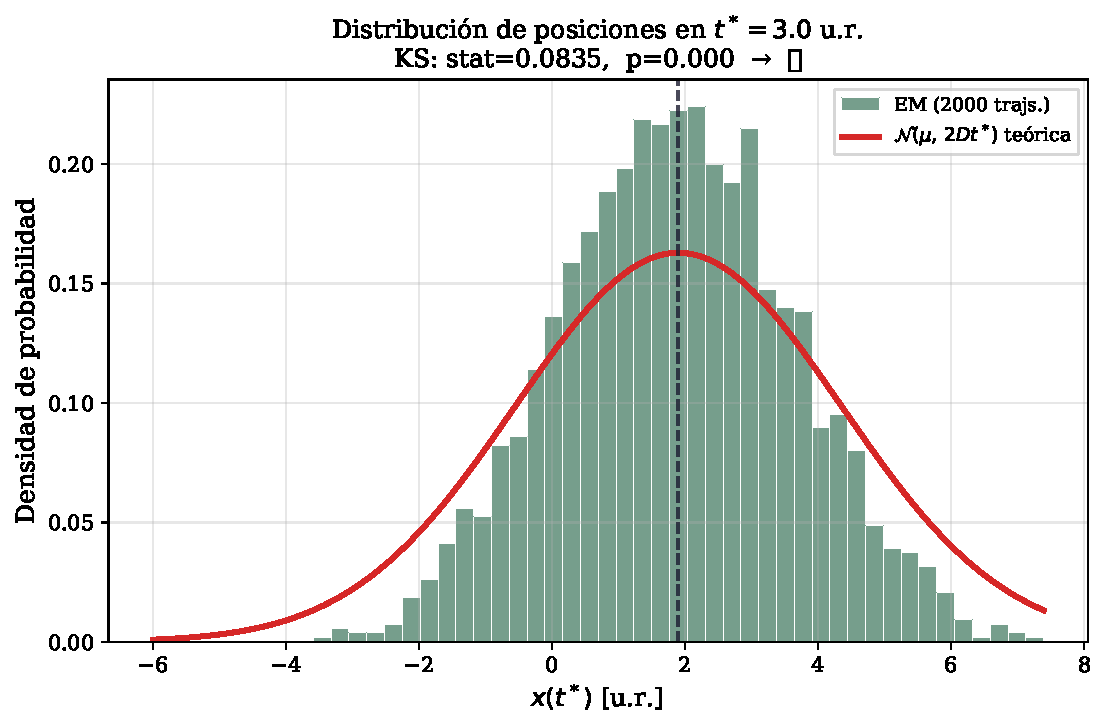
\includegraphics[width=\columnwidth]{fig_histograma.pdf}
	\caption{Position histogram at $t^*=3$\,r.u.\ (green) and
		theoretical Gaussian $\mathcal{N}(\mu_{\rm teo},\sqrt{2Dt^*})$
		(red). $\mu_{\rm teo}=1.900$, $\sigma_{\rm teo}=2.449$.}
	\label{fig:hist}
\end{figure}

\paragraph{Velocity autocorrelation and spectral analysis.}
Figure~\ref{fig:acv} compares the velocity autocorrelation function
(VACF) computed over the ensemble with the analytical prediction
$C_v(\tau)=e^{-\beta\tau}$.  Agreement is excellent for
$\tau\lesssim5\tau_{\rm rel}$; deviations at long lags are attributable
to statistical noise $\sim1/\sqrt{N}$.  The numerical integral
$D_{\rm GK}=\int_0^\infty C_v(\tau)\,\frac{\kB T}{m}\,d\tau$ is
consistent with the MSD value.
The power spectral density (PSD) of $\xi(t)$ (Fig.~\ref{fig:fft}),
estimated by the Welch method over 200 trajectories, is approximately
constant for $f<f_c=\beta/(2\pi)$, confirming the white-noise character
in the relevant frequency range.  At high frequencies ($f\gg f_c$) the
damped oscillator response acts as a low-pass filter $\propto f^{-2}$.

\begin{figure}[h!]
	\centering
	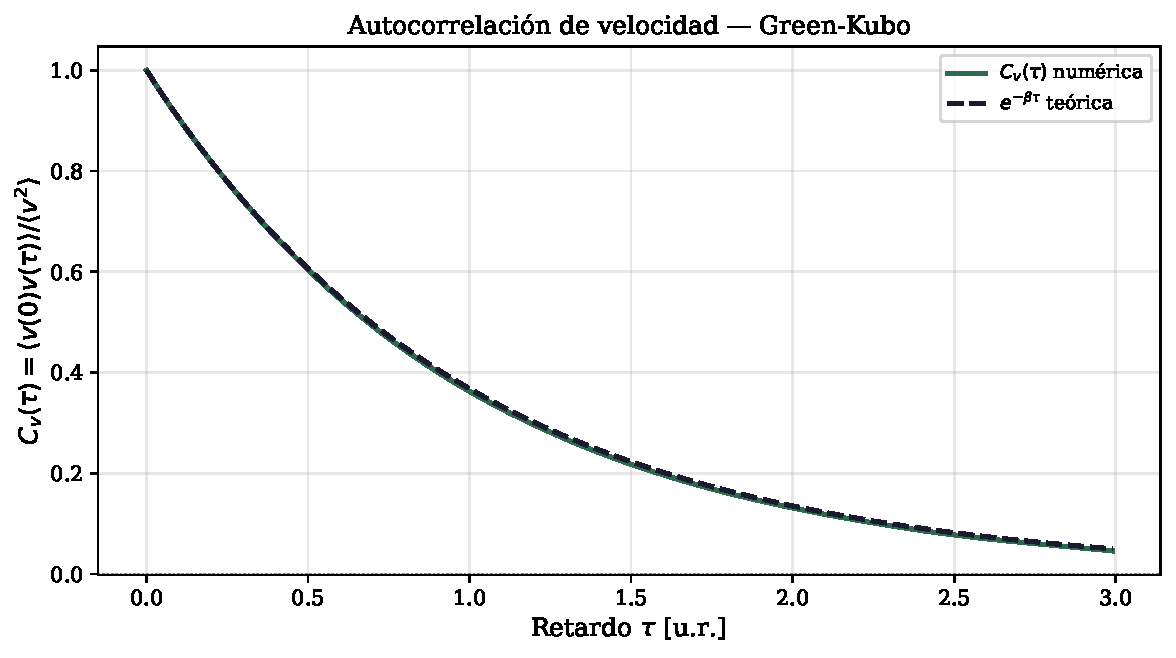
\includegraphics[width=\columnwidth]{fig_autocorr.pdf}
	\caption{Normalized velocity autocorrelation. Green: numerical
		(EM ensemble); dashed black: analytical $e^{-\beta\tau}$.}
	\label{fig:acv}
\end{figure}

\begin{figure}[h!]
	\centering
	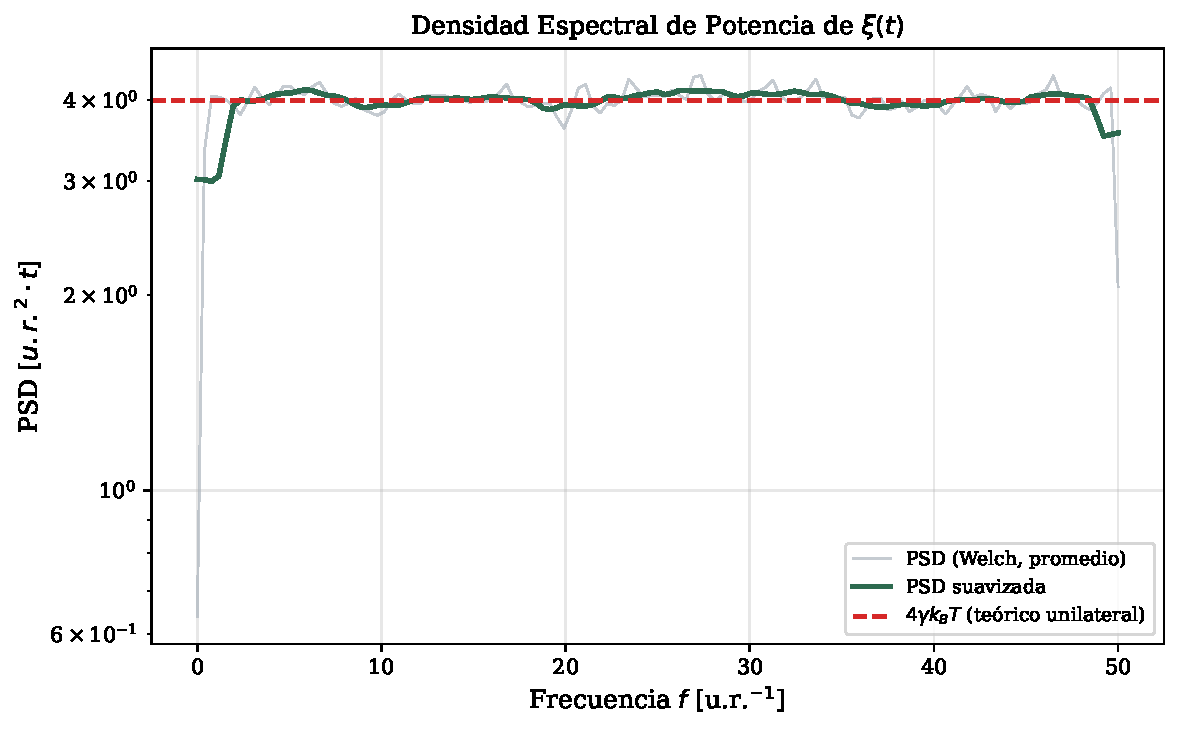
\includegraphics[width=\columnwidth]{fig_fft.pdf}
	\caption{PSD of $\xi(t)$ (log scale). Gray: individual spectrum;
		green: smoothed Welch average; dashed red: theoretical value
		$4\gamma\kB T$ (one-sided PSD).}
	\label{fig:fft}
\end{figure}

\paragraph{Parametric dependence.}
Figure~\ref{fig:Tparam} shows the MSD for four temperatures
$T\in\{0.5,\,1,\,2,\,4\}$.  The slope scales linearly with $T$,
confirming $D\propto T$.

\begin{figure}[h!]
	\centering
	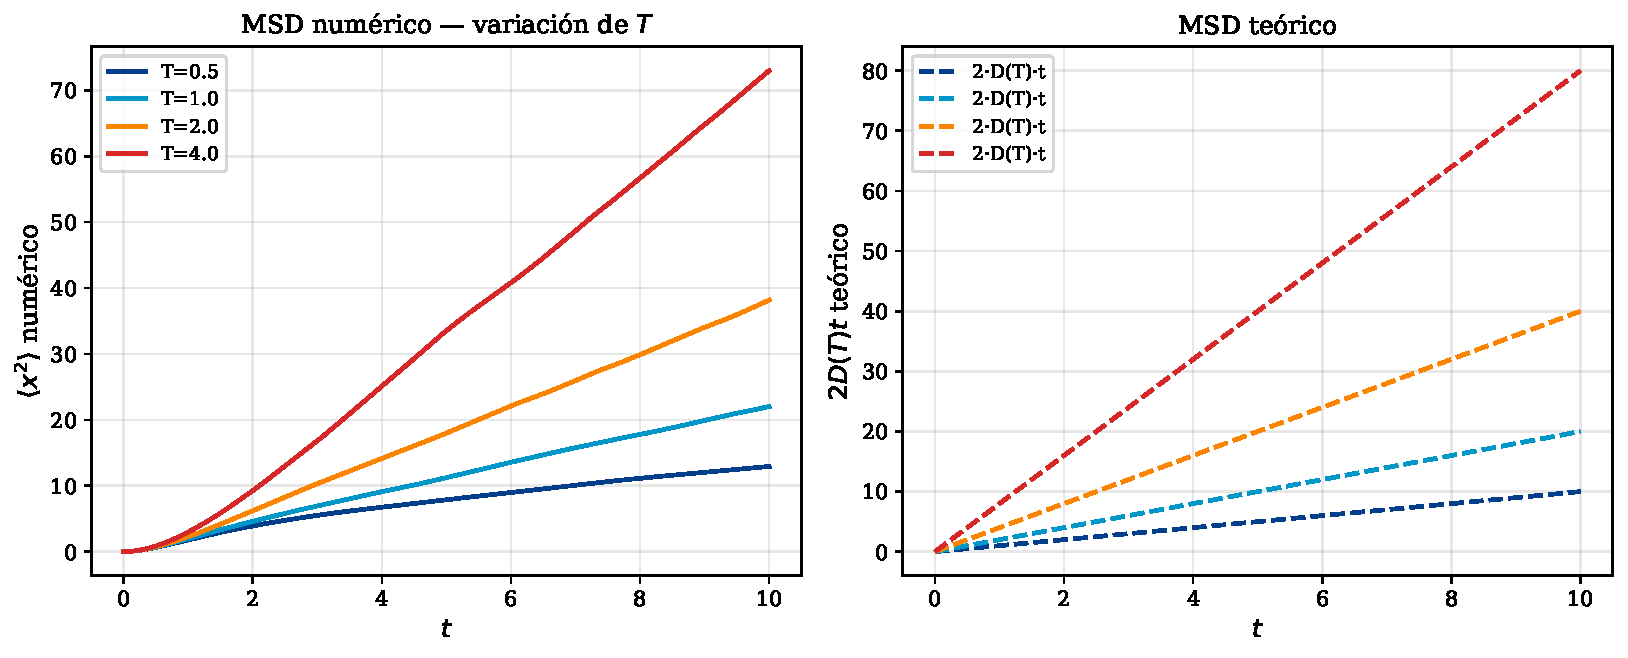
\includegraphics[width=\columnwidth]{fig_parametrico_T.pdf}
	\caption{Numerical (left) and theoretical $2D(T)t$ (right) MSD for
		four temperatures.  Diffusivity increases linearly with $T$ in
		agreement with $D=\kB T/\gamma$.}
	\label{fig:Tparam}
\end{figure}
\newpage
% ============================================================
\section{Discussion}
\label{sec:discusion}
% ============================================================

The convergence analysis quantitatively confirms the superiority of
RK4 in the deterministic case: for equal $\dt$, the RK4 error is
$\sim8$ orders of magnitude smaller than that of Euler.  However, this
benefit comes at the cost of four evaluations of $f$ per step versus
one for Euler, making the per-step cost of RK4 roughly $4\times$
higher.  In practice, using RK4 with a step $\sim10\times$ larger
maintains the same accuracy at the same computational cost as Euler.

In the stochastic case, applying RK4 directly to an SDE does not
improve convergence beyond the order $1/2$ of EM~\cite{Kloeden1992},
since the intermediate stages require evaluating $dW$ over
sub-intervals with no support in higher-order Itô/Stratonovich
calculus~\cite{Leimkuhler2015}.  EM is therefore the formally correct
choice.

For $t\ll\tau=m/\gamma$ the motion is approximately rectilinear
(\textit{ballistic regime}): $\MSD\approx v_T^2 t^2$ with
$v_T^2=\kB T/m$.  The crossover to the diffusive regime ($\MSD=2Dt$)
occurs around $t\sim\tau$.  Increasing $m$ lengthens $\tau$ and makes
the ballistic regime more prominent; increasing $\gamma$ shortens it.

The spectral verification shows that the PSD of $\xi$ satisfies the
FDR~\eqref{eq:fdr}: the spectrum is flat with amplitude
$\propto\gamma T$ in the relevant range.  Deviations at high
frequencies are discretization artifacts that vanish as $\dt$ is
reduced.

% ============================================================
\section{Conclusions}
\label{sec:conclusiones}
% ============================================================

This work presents a quantitative validation of three integrators for
the Langevin equation in both the deterministic and stochastic regimes.
In the deterministic setting, the hierarchy of precision between Euler
and RK4 is clearly established: the measured convergence orders
reproduce the theoretical predictions with errors below $0.5\%$.
This accuracy advantage does not carry over to the stochastic regime:
the non-differentiable nature of the Wiener process imposes a strong
convergence ceiling of order $1/2$ that is independent of the
deterministic scheme employed, making EM the formally correct choice
for Itô SDEs.

Ensemble simulation with EM satisfactorily verifies the physics
predicted by Einstein's theory: the linear diffusion law is confirmed,
the velocity autocorrelation follows the exponential decay expected
from the Green-Kubo relation, and the spectral analysis confirms the
consistency of the implementation with the fluctuation-dissipation
relation.  Taken together, the results underscore that the choice of
integrator must be guided by the mathematical nature of the noise and
not solely by the accuracy of the deterministic part.

Natural extensions include Brownian motion under external potentials
(the Ornstein-Uhlenbeck process), dynamics in higher dimensions,
fractional Brownian motion, and the implementation of higher-order
methods such as Milstein or stochastic Runge-Kutta of order~1.

% ============================================================


% ============================================================
\bibliography{referencias}

\end{document}
